\section{Goursat's Theorem}

\begin{theorem}[Goursat's Theorem]\label{4.8.1}
    Let $G$ be open in  $\C$ and  $f:G \xrightarrow{} \C$ a complex
    differentiable function. Then $f$ is holomorphic on $G$.
\end{theorem}
\begin{proof}
    Suppose, without loss of generality, that $G$ is an open ball. Let
    $T=[a,b,c,a]$ and $\Delta$ the closed set formed by $T$ and $\Int{T}$; that
    is, $T=\partial{\Detla}$.

    \begin{figure}[h]
        \centering
        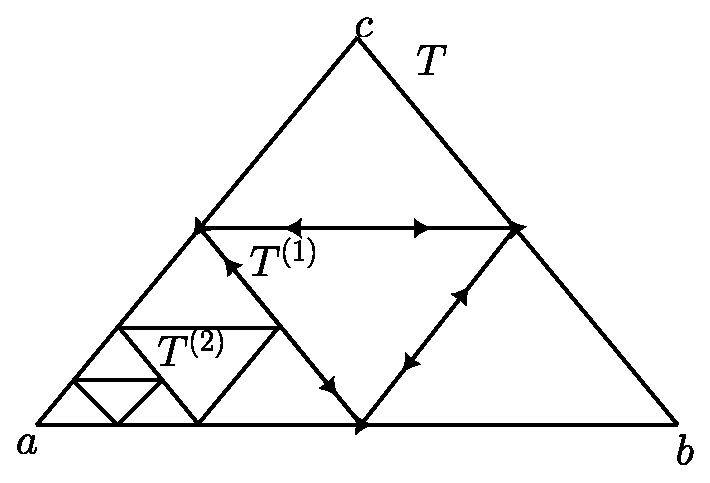
\includegraphics[scale=0.5]{Figures/Chapter4/goursat_triangle.eps}
        \caption{}
        \label{figure_4.5}
    \end{figure}

    Now, choose the midpints on the sides of $\Delta$ to form the triangles
    $\Delta_1$, $\Delta_2$, $\Delta_3$, and $\Delta_4$, and the paths $T_j$ such
    that  $T_j=\partial{\Delta_j}$, for $j=1,2,3,4$. Then notice that
    \begin{equation*}
        \int_T{f}=\sum_{j=1}^4{\int_{T_j}{f}}
    \end{equation*}
    Now, among these paths, there is a path $T^{(1)}$ such that
    \begin{equation*}
        \Big{|} \int_T{f} \Big{|} \leq \Big{|} \int_{T(1)}{f} \Big{|}
    \end{equation*}
    moreover, notice that $l(T_j)=\frac{1}{2}l(T)$, and
    $\diam{\Delta_j}=\frac{1}{2}\diam{\Delta}$. So we get
    \begin{equation*}
        \Big{|} \int_T{f} \Big{|} \leq 4\Big{|} \int_{T^{(1)}}{f} \Big{|}
    \end{equation*}

    Now, proceed agaain on $T^{(1)}$ and obtain a path $T^{(2)}$ with
    \begin{equation*}
        \Big{|} \int_{T^{(1)}}{f} \Big{|} \leq 4\Big{|} \int_{T^{(2)}}{f} \Big{|}
    \end{equation*}
    Proceeding recursively (See figure \ref{figure_4.5}), we obtain a sequence
    $\{T^{(n)}\}$ of closed triangular paths such that if
    $T^{(n)}=\partial{\Delta^{(n)}}$, then
    \begin{equation*}
        \dots \subseteq \Delta^{(2)} \subseteq \Delta^{(1)} \subseteq \Delta
    \end{equation*}
    and
    \begin{equation*}
        \Big{|} \int_{T^{(n)}}{f} \Big{|} \leq 4\Big{|} \int_{T^{(n+1)}}{f} \Big{|}
    \end{equation*}
    with
    \begin{equation*}
        l(T^{(n+1)})=\frac{1}{2}l(T^{(n)}) \text{ and }
        \diam{\Delta^{(n+1)}}=\frac{1}{2}\diam{\Delta^{(n)}}
    \end{equation*}
    Therefore, we get
    \begin{equation*}
        \Big{|} \int_{T^{(n)}}{f} \Big{|} \leq 4^n\Big{|} \int_T{f} \Big{|}
    \end{equation*}
    and
    \begin{equation*}
        l(T^{(n+1)})=\frac{1}{2^n}l(T) \text{ and }
        \diam{\Delta^{(n+1)}}=\frac{1}{2^n}\diam{\Delta}
    \end{equation*}
    Now, since each $\Delta^{(n)}$ is closed, by Cantor's theorem (theorem
    \ref{2.3.4}), we have
    \begin{equation*}
        \bigcap{\Delta^{(n)}}=\{z_0\}
    \end{equation*}

    Now, let $\e>0$, since  $f$ has a derivative at  $z_0$, choose a $\d>0$ such
    that  $B(z_0,\d) \subseteq G$, and
    \begin{equation*}
        \Big{|} \frac{f(z)-f(z_0)}{z-z_0}-f'(z_0) \Big{|}<\e \text{ whenever }
        0<|z-z_0|<\d
    \end{equation*}
    Alternatively, we get
    \begin{equation*}
        |f(z)-f(z_0)-f'(z_0)(z-z_0)| \leq \e|z-z_0| \text{ whenever }
        0<|z-z_0|<\d
    \end{equation*}
    Choose, then an $n \in \Z^+$ for which
    $\diam{\Delta^{(n)}}=\frac{1}{2^n}\diam{\Delta}<\d$. Since $z_0 \in
    \Delta^{(n)}$, we get that $\Delta^{(n)} \subseteq B(z_0,\d)$. Then by
    Cauchy's theorem, we get
    \begin{equation*}
        \int_{T^{(n)}{dz}}=\int_{T^{(n)}{z \ dz}}=0
    \end{equation*}
    hence
    \begin{equation*}
        \Big{|} \int_{T^{(n)}{f}} \Big{|}=
        \Big{|} \int_{T^{(n)}{(f(z)-f(z_0)-f'(z_0)(z-z_0)) \ dz}} \Big{|} \leq
        \e\int_{T^{(n)}}{|z-z_0| \ |dz|} \leq \e{l(T)}\diam{\Delta} \leq
        \e\frac{1}{4^n}l(T)\diam{\Delta}
    \end{equation*}
    This gives
    \begin{equation*}
        \Big{|} \int_T{f} \Big{|} \leq \e{l(T)}\diam{\Delta}
    \end{equation*}
    since $\e$ is arbitrary, this gives us $\int_T{f}=0$. By Morera's theorem,
    this makes $f$ holomorphic on $G$.
\end{proof}
